\section{Architecture}

\begin{figure}[ht]
  \centering
  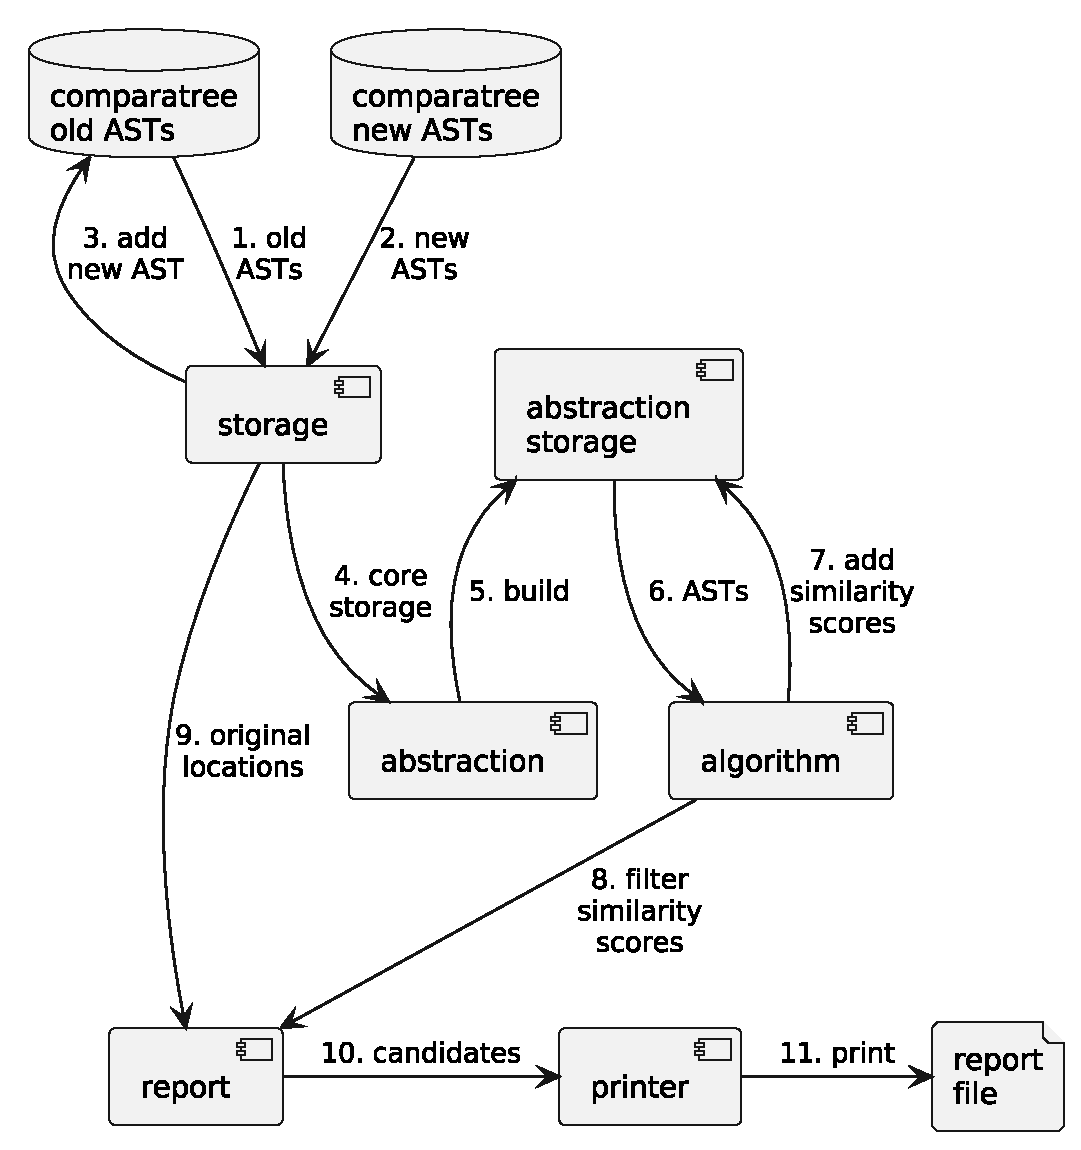
\includegraphics[width=\textwidth]{img/contrast-flow.eps}
  \caption{Data flow of \texttt{ContrAST}.}
  \label{fig:contrast-flow}
\end{figure}

The data flow of \texttt{ContrAST} is shown in \autoref{fig:contrast-flow}.
\begin{itemize}
\item \texttt{storage} provides access to the \texttt{comparatree} instances and their ASTs. It merges all the instances into a single \texttt{comparatree} archive, keeping all the indices from the archive intact.
\item \texttt{abstraction} builds a new core storage from the \texttt{storage}, simplifying the original labels and removing unnecessary information.
\item \texttt{abstraction storage} is a simplified version of the \texttt{storage}, keeping links between the original ASTs and their simplified versions.
\item \texttt{algorithm} compares the ASTs from the \texttt{abstraction storage}, saves the similarity scores back to the \texttt{abstraction storage}, and creates a report with the found results and their similarity scores.
\item \texttt{printer} prints the report to a file in a chosen format.
\end{itemize}

Note how separated the activities of the components are.
The \texttt{storage} can be loaded and saved independently of the rest of the system.
The \texttt{algorithm} can only compute similarity scores and save them without the need to immediately create one specific report.
The \texttt{printer} can ask \texttt{algorithm} for the report and print it without the need to compute the similarity scores again.

All the components have their settings and configuration options, allowing for easy customization of the tool.
We integrated the \texttt{CLI11} \cite{cli11} library for command-line parsing.
It loads the settings from the command-line arguments, and we can then create the components with the given settings.

There is a global \texttt{registry} that keeps track of all available switchable components, allowing for easy replacement of the components with different implementations.
The switchable components are \texttt{abstraction}, \texttt{algorithm}, and \texttt{printer}, and we can get an instance of any of them from the \texttt{registry} by specifying the name of the desired implementation.
